\documentclass[12pt,a4paper, oneside]{article}

\usepackage[top=2.5cm, bottom=2.5cm,left=3.50cm,right=2cm]{geometry}

\usepackage{graphicx}

%--------line spacing------------
\renewcommand{\baselinestretch}{1.5}

\usepackage{datetime}

\newdateformat{monthyeardate}{%
	\monthname[\THEMONTH], \THEYEAR}

\usepackage[centertags]{amsmath}
\usepackage{amsfonts}
\usepackage[tracking=true]{microtype}
\usepackage[framemethod=TikZ]{mdframed}
\usepackage{multirow,url}
\usepackage{amssymb}
\usepackage{mathtools,makecell,pbox,booktabs}
\usepackage{amsthm}
\usepackage{newlfont}
\usepackage{fancyhdr,enumitem}
\usepackage{subfigure}
%\usepackage{expl3}
%\usepackage{l3backend}
\usepackage{longtable}
\usepackage{rotating}
\usepackage{breqn}
%\usepackage{glossary}
\usepackage{subfigure}
\usepackage{times}
\usepackage{setspace}
\usepackage{color}
\usepackage{amsmath}
\usepackage[linesnumbered,ruled]{algorithm2e}
\usepackage{algcompatible}
%\usepackage{vector}
\usepackage{lscape}
\usepackage{caption}
\usepackage{titlesec}
\usepackage{longtable}
\usepackage[square,comma,numbers,sort&compress]{natbib}
\begin{document}
%\include{front_page} %correct
\begin{titlepage}
\newgeometry{left=2.5cm,right=2cm,top=2cm,bottom=1.25cm}
%\vspace{-1.0cm}
\newcommand\narrowstyle{\SetTracking{encoding=*}{-29}\lsstyle}
\title{ABCD}
\renewcommand{\baselinestretch}{1.5}
 \setlength{\parindent}{0pt}


%\textheight = 630pt \topmargin=0pt \voffset=1cm \headheight = 0pt
%\marginparwidth= 0pt \headsep = 0pt

\pagestyle{empty}
	\narrowstyle{
\begin{center}
%\textbf{A}\\
%\textbf{Thesis} \\
%\textbf{on}\\
%\vspace{.8cm}
%\vspace{-2pt}
\begin{singlespace*}
	\begingroup
 	\vspace{-2.0cm}
 	\centering
 	{\Large {\it A \\Synopsis Report \\on} \par}
 	\vspace{0.5cm}
 	{\LARGE\bfseries Tomato Leaf Disease Detection \par}
 	\vspace{0.6cm}
 	{\Large\itshape submitted in partial fulfillment of the requirements \\for completion of AI LAB\\of \par}
 	\vspace{0.2cm}
 	{\Large\bfseries TY COMP \par}
 	% 	\vspace{0.2cm}
 	{\Large\itshape in \par}
 	% 	\vspace{0.2cm}
 	{\Large\bfseries Computer Engineering \par}
 	\vspace{0.2cm}
 	{\Large\itshape by \par}
 	\vspace{0.5cm}
 	{\Large\bfseries Kedar Adkine (112003003) \par}
 	{\Large\bfseries Gourav Bangad (112003014) \par}
   	{\Large\bfseries Param Barge (112003015) \par}
 	%\vspace{0.2cm}
 	\vspace{0.7cm}
 	{\Large\itshape Under the guidance of \par}
 	\vspace{0.9cm}
 	{\Large\bfseries  Prof. Suraj Sawant \par}
 	%\vspace{0.2cm}
 	%{\Large \itshape Professor \par}
 	%\vspace{0.2cm}
 	{\Large \itshape Department of Computer Engineering \par}
 	\vspace{0.5cm}
 	
\includegraphics[width=0.2\textwidth]{images/coeplogo.jpg}
 	\par
 	\vspace{0.5cm}
 	{\Large Department of Computer Engineering, \par}
 	{\Large COEP Technological University (COEP Tech) \par
         (A Unitary Public University of Govt. of Maharashtra)  \par}
 	{\Large Shivajinagar, Pune-411005,Maharashtra, INDIA \par}
 	\par
 	\vspace{0.2cm}
 	% 	\vfill
 	% 	\vfill
 	% Bottom of the page
 	{\large \monthyeardate\today\par}
	\endgroup
\end{singlespace*}


\end{center}
}
\end{titlepage}
%\clearpage  
\restoregeometry%correct
\section{\underline{Abstract}}
\textbf{\emph{The study described in this paper consists of a method that uses Support Vector Machines (SVMs) alongwith neural network functions in order to detect and identify type of disease that infects tomato plant.In this project, we used dataset consisting of images of tomato leaves.Supported Vector Machines technique has been employed to identify an optimal feature subset. Finally, a support vector machine classier with different neural network algorithms was employed to evaluate the ability of this approach to detect and identify where tomato leaf infected with Bacterial spot, early blight, Septoria leaf spot, etc. To evaluate the performance of presented approach, we tested our proposed model on dataset consisted of 10000 images comprised of 10 types of tomato leaf diseases. Extensive experimental results demonstrate that the proposed approach provides excellent annotation with accuracy more than 80\%. Efficient result obtained from the proposed model can lead to tighter connection between agriculture reasearchers and computer technology, yielding more effective and reliable results.
}}

\newpage



\begin{figure}
\section{\underline{Introduction}}

    
    \begin{center}
    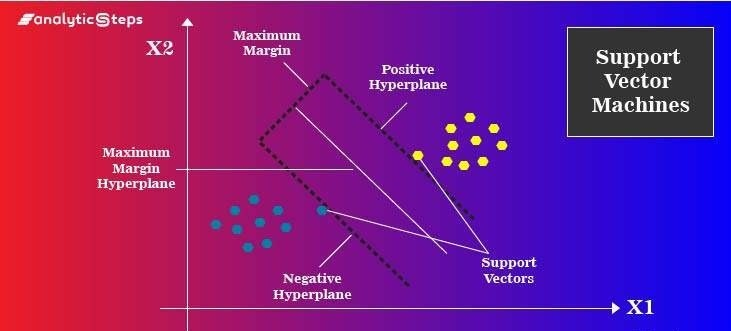
\includegraphics[width=400]{images/intro.jpg}
    \caption{SVM}
\end{center}
\end{figure}

\\
\setlength{\parindent}{20pt}    Tomatoes are one of the most widely cultivated food crops throughout the world due to its high nutritive value. It contains a lot of vitamins and nutrients such that vitamin C. It occupies the fourth level between word vegetables. Although, the naked eye observation of experts is the main approach adopted in practice for detection and identification of plant diseases, it requires continuous monitoring of experts, which might be expensive and difficult especially in large farms. So, it is necessary to help farmers in automatically detect symptoms of disease as soon as they appear by analyzing the digital images. Aiming at minimizing economic losses, ensuring both quality and quantity of agricultural products and minimizing agrochemicals use, computer based applications have been developed and revealed high efficacy. In this paper, a combination of various machine intelligence techniques has been used to detect diseased tomato leaf for the purpose of diagnosing pathogen types that infect tomato. The proposed SVM-based tomato diseases detection approach utilizes some preprocessing techniques such that image cropping and image filtering for improving the quality of leaf images.


\pagebreak
\begin{figure}


\section{\underline{Motivation}}
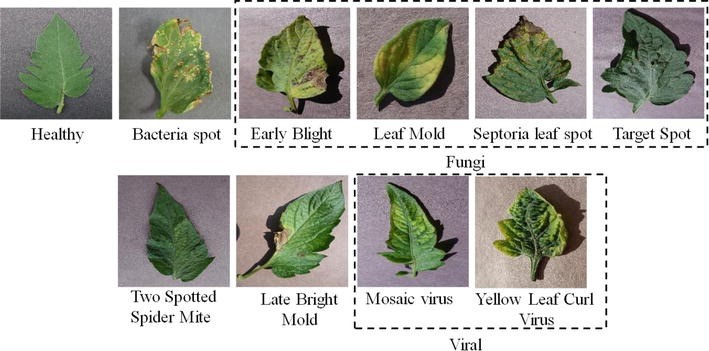
\includegraphics[width=450]{images/motivation.jpg}
\caption{Tomato leaves with various diseases}
\end{figure}\\
Tomato, worldwide, is infected by several viral diseases which cause stunting, leaf curl, yellowing, mosaic, mottling, necrosis and shoe-string symptoms on plants, leaves or fruits. Among them, bud necrosis disease caused by an orthotospovirus is emerging as a major constraint to the cultivation of tomato for resource-poor farmers. In the Indo-Gangetic eastern plains, various disease incidence on tomato ranged from 0 to 45\% under field conditions during 2015 and 2016, along with other diseases such as leaf curl and mosaic (0–35\%) and target spot (0–18\%) respectively. Thirty four viral infected samples collected from 11 different villages were screened for different viruses using serological and PCR-based methods. The result revealed that most samples were positive for RNA (leaf curl virus, tomato mosaic virus). So, in order to stop the spread of such type of harmful diseases, our model accurately predicts which type of disease crop is going through with and help farmer take appropriate precautions.

\pagebreak
\begin{figure}
\section{\underline{ Literature Review}}
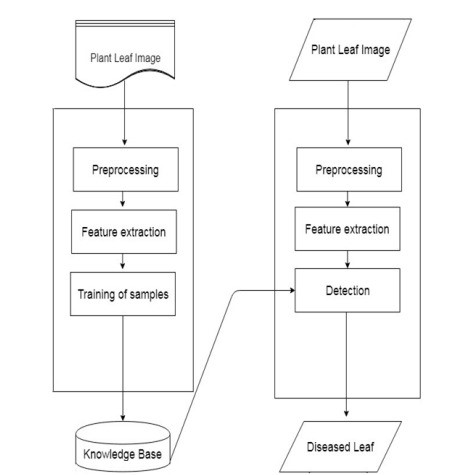
\includegraphics[width=450,height=350]{images/LR.jpg}
\caption{Flow chart for model}
\end{figure}\\
Support vector machine (SVM) is a classification technique originally developed by Vapnik. It was recently used in many applications including pattern recognition, bioinformatics, cancer diagnosis. It tries to find the trade-off between minimizing the training set error and maximizing the margin, to achieve the best generalization ability and remains resistant to over fitting. SVM works by mapping data to a high-dimensional feature space, so that data points can be categorized, even when the data are not otherwise linearly separable. SVM uses a nonlinear mapping to transform the original training data into a higher dimension, then it searches to and a linear optimal hyperplane, so that the margin of separation between the two classes is maximized.

\pagebreak


\section{\underline{Research Gaps}}
\begin{enumerate}
    \item The main motive behind the project is to detect disease in tomato leaf. This further can extended to enhancing the model which will be capable of answering the cause and solution for the particular disease.
    \item This can be achieved by suggesting the name of pest that caused particular disease and name of pesticide that is used for the remedy of the disease.
    \item It will require large dataset consisting of pests, pesticides along with leaf images for making appropriate predictions of the disease.
    \item Efficient result obtained from the proposed approach can lead to tighter connection between agriculture specialists and computer system, yielding more effective and reliable results.
\end{enumerate}






\section{\underline{Problem Statement and Objectives}}
\begin{enumerate}
    \item Our primary objective of this project is to develop a model to categorize
input plant leaf pictures as healthy or unhealthy. Moreover the objective of the proposed method is to develop a technique to identify leaf disease in tomato plant by improving the classification accuracy and reducing computational time.
    \item In this project, we are trying to help farmers by solving the issue regarding the early detection of tomato leaf diseases so that they can start preparing for prevention of diseases. Thus 
    minimizing their economic losses.
    \item This proposed model is a self-learning model. We aim to imporve the accuracy of prediction made by model as much as possible. It can be achieved by testing more number of images ensuring an accurate prediction.
    
\end{itemize}

\newpage

\begin{figure}
\section{\underline{Methodology}}




\textbf {Support Vector Machine (SVM) classifier : } \\
To classify the various diseases in plants any of the machine 
learning techniques can be used. The classification phase 
suggested deciding if the input image is healthy or diseased. 
In this paper Support Vector Machine (SVM) classifier has 
been used because it has some advantages over other 
classifiers such as effective in high dimensional spaces also in 
cases where the number of dimensions is greater than the 
number of samples. It is memory efficient as it uses a subset 
of training points in the \textbf{decision function} (called \textbf{support 
vectors}). \\
{SVM }is a supervised machine learning algorithm used for 
both classification and regression. SVM is a discriminative 
classifier. In this approach, for classification, the SVM 
technique has been applied. In SVM, each data item is plotted 
as a point in n-dimensional space; the number of dimensions 
corresponding to the number of features being classified. The 
classification is obtained by discovering the hyper-plane that 
uniquely distinguishes between different groups of scattered 
data points. By finding the hyper-plane the classification is 
performed. Hyper-plane differentiates two classes very well. 
This is shown in Figure 4.
\begin{center}

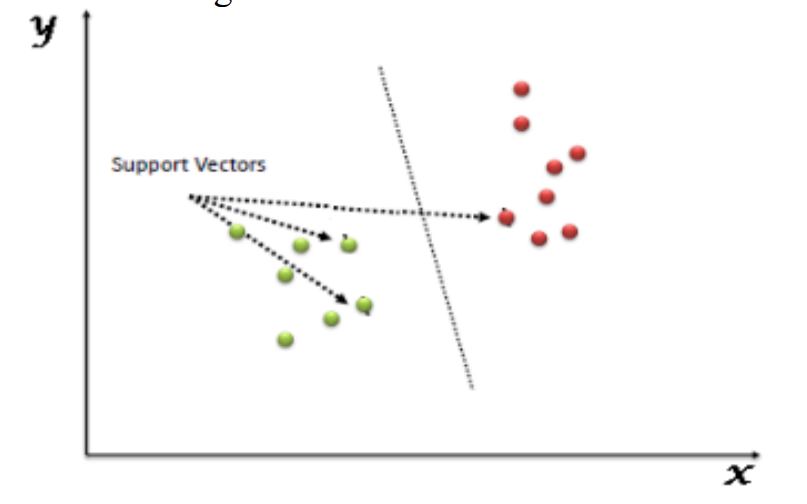
\includegraphics[width=250]{images/Screenshot (155).png}
\caption{Classification of healthy (in green) and diseased part of leaf (in red)}

\end{center}
\end{figure}


\pagebreak
\begin{figure}
{\centering

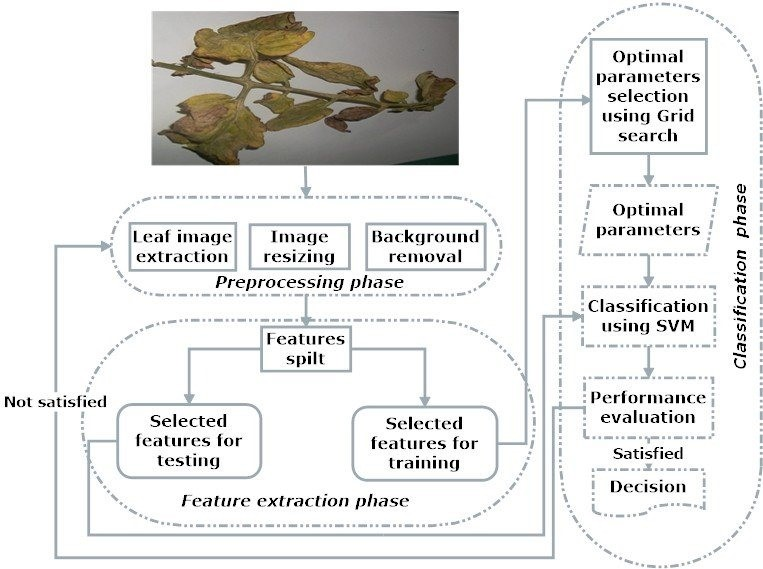
\includegraphics[width=400,height=250]{images/methodology.jpg}
    
\caption{Prediction Process of disease}
\end{figure}

}

The proposed SVM-based tomato diseases detection approach is comprised of the following four fundamental building phases : 
\begin{enumerate}
    \item \textbf{Image acquisition phase :}  The proposed SVMbased tomato diseases detection approach begins with acquiring and collecting digital images from suitable environment.
    \item \textbf{Pre-processing phase :}  To improve the quality of the images and to make the feature extraction phase more reliable prepare, some image-processing techniques are applied including leaf image isolation, image resizing and background removing.
    \item \textbf{Feature extraction phase : } 402 texture-based features have been extracted, and represented in a database as vector values.
    \pagebreak
    \item  \textbf{Classification phase : }   The last phase is the classification and prediction of new objects, it is dependent on the SVM classifier. These four phases are described in detail in the following subsections and depicted in Figure 5.
\end{enumerate}

\newpage

\section{\underline{Hardware and Software Requirements}}
The proposed model must be able to detect disease. The performance will depend upon GPU power. Users can follow up the interface step by step for their purpose. The proposed model must be available for use to the user as and when needed provided that the user’s system meets the specified requirements. The proposed system must be able to recover from failure in case of the application crashing abruptly and become ready-to-use after recovery. Along with the necessary peripheral hardware, and Python 3 will be used to implement the software functionality of drowsiness detection.\\
\begin{itemize}
    \item \textbf{\underline{Software Requirements:}}
python3, Tensorflow 2.10.0, Keras 2.10.0, NumPy 1.23.4, \\
Panda 1.5.1
\item \textbf{\underline{Hardware Requirements:}}
NVIDIA-SMI 472.19, Driver Version : 472.19, CUDA Version : 11.4,    GPU Name : TCC/WDDM.
\end{itemize}



\section{\underline{Conclusions}}

In this paper, an effective SVM-based tomato leaf diseases detection approach is proposed to recognize two types of tomatoes leaf diseases. The dataset consists of in total 11000 (10000 images-training dataset and 1000 images-testing dataset) infected tomato leaf images with Bacterial spot, early blight, etc were used for both training and testing phase. Overall validation accuracy (after 10th epoch) is 82.93\% whereas training accuracy is 89.30\%.


\begin{figure}

\section{\underline{Timeline Chart}}
    \begin{center}
        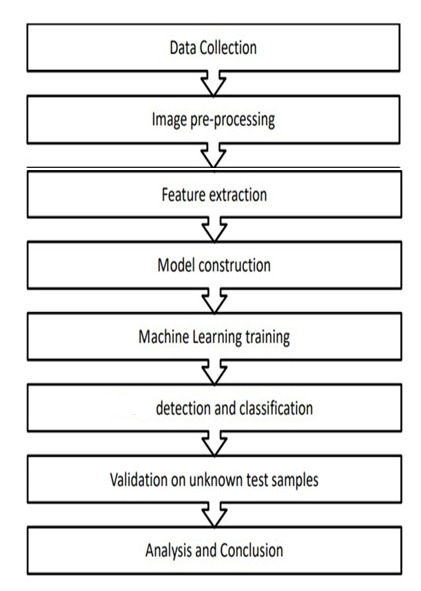
\includegraphics{images/Flowchart_1.jpeg}
        \caption{Flowchart for design and development of proposed model}
    \end{center}
\end{figure}


\newpage

\bibliographystyle{IEEEtran}
\bibliography{citation}
\end{document}